Answering \ref{rq:2}, this chapter presents a proposal for the engineering of \emph{Heterogeneous} \acp{DTE} (\Cref{chap:dte:dte}).
%
Motivated by the design of the Web and its success in creating interoperability among digital services---more recently, in \ac{IoT} systems through the \ac{WoT} (\Cref{chap:back:Web})---the chapter explores whether and to what extent hypermedia principles and Web standards can be applied to design and implement \acp{DTE}. 
%
The result of this investigation, refines and extend the ideas originally presented in \cite{web-of-dt-ricci-2022}, combining the \ac{WoDT} conceptual model with the design rationale of the Web to build a \emph{\ac{HWoDT}}.

This approach offers a practical implementation strategy for \acp{DTE}, enabling interoperability at both the \ac{DT} and ecosystem levels, and facilitating uniform interaction across \acp{DT} regardless of the underlying technological stack.

The chapter presents the \ac{HWoDT} conceptual integration of hypermedia principles and Web standards in \ac{DTE}, 
and the prototype implementation of a supporting set of tools that demonstrate the feasibility of the approach.


%======================================================
\section{A \acl{HWoDT}}
\label{sec:hwodt-idea}
%======================================================

The main driver of the proposed approach is to support seamless integration of existing \acp{DT}, regardless of their underlying technologies and with minimal overhead.
%
Hence, the core idea is to hide the heterogeneity of \acp{DT} behind a \emph{uniform interface} built with Web protocols and standards, and supported by an explicit semantic layer that allows \acp{DT} to provide a uniform description of both their state and their features and services. 
%
Thus, the name \emph{\acf{HWoDT}}, aims to emphasize the hypermedia-driven nature of the approach, following the \ac{HATEOAS} principle of the \ac{REST} architectural style~\cite{fielding2000architectural}.

Such an interoperability layer enables navigation and seamless interaction with heterogeneous \acp{DT}.
%
To complement it with additional ecosystem-level functionalities, the idea of a \emph{WoDT Platform} is introduced as both a scope boundary defining ecosystem membership and an aggregation layer enabling consumers to query, observe, and exploit services across distributed \acp{DT}.

As illustrated in \Cref{fig:hwodt}, the resulting architecture is composed of \acp{DT}:
\begin{inlinelist}
    \item created using heterogeneous technologies,
    \item implementing the uniform interface through \emph{adapters},
    \item connected by relationships that reflect the physical ones,
    \item and that are aggregated into \acp{DTE} by being registered to one or multiple WoDT Platforms.
\end{inlinelist}    

\begin{figure}[t]
  \centering
  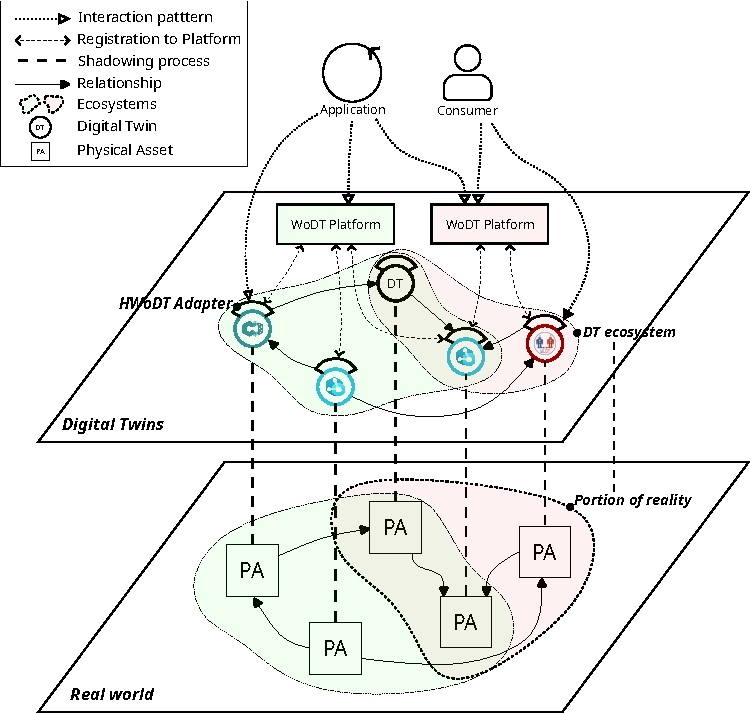
\includegraphics[width=0.7\columnwidth]{figures/hwodt/hwodt.pdf}
  \caption{The Hypermedia WoDT scheme, in the real world PAs (squares) belonging to different organizations and domains are connected by relationships. In the digital world, cross-domain ecosystems of DTs (circles) mirror different portions of reality, supported by the WoDT Platform.}
  \label{fig:hwodt}
\end{figure}

%-----------------------------------------------------------
\subsection{A Uniform Interface for Heterogeneous DTs}
\label{ssec:uniform-interface}
%-----------------------------------------------------------

The first step towards integrating heterogeneous \acp{DT} is to look into how each individual \ac{DT} can expose a uniform interface, compliant with the requirements of the \ac{HWoDT}.
Achieving standard semantic representations of \acp{DT} is an open challenge for the \ac{DT} community.
%
In this work, adopting a pragmatic approach, the benefits of uniform semantic representations in building interoperability are demonstrated through a proposal grounded on the \ac{HATEOAS} principle of the Web architecture:
each \ac{DT} must be able to provide consumers with both \emph{data} and \emph{affordances}---i.e., action possibilities---through hypermedia representations.
This leads to distinguish two logically different representations:
\begin{itemize}
    \item a \emph{\acf{DTD}}, inspired by the \ac{WoT} \acl{TD}, to hold metadata and affordances, enabling consumers to understand the \ac{DT} model, as well as which services the \ac{DT} exposes and how to access them;
    \item a \emph{\acf{DTKG}} representing the live state of the \ac{DT}, semantically encoding domain knowledge and supporting state observation, querying, and discovering relationships between \acp{DT}.
\end{itemize}

Each \ac{DT} is further required to comply with a set of standard \emph{interaction patterns} to allow consumers to uniformly obtain and manipulate such representations for all \acp{DT} in the \ac{HWoDT}.

%.................................
\subsubsection{The \acl{DTD}}
%.................................

The \ac{DTD} serves the primary purpose of providing management metadata about a \ac{DT}, registering it within the ecosystem and describing the exposed interactions\footnote{Documentation on the structure of the \ac{DTD} schema is available on GitHub \url{https://github.com/Web-of-Digital-Twins/dtd-conceptual-model}}.

A primary concern is \emph{identification} of the \ac{DT} and the associated \ac{PA} to unambiguously distinguish them from other elements of the ecosystem.
While \acp{PA} may use domain-specific identifiers (e.g., a serial number), each \ac{DT} in a \ac{HWoDT} is identified with a persistent, globally unique \ac{URI}.
This ensures identification and accessibility of \acp{DT} as Web resources throughout their whole lifecycle.

Furthermore, to support navigation from a \ac{DT} to the ecosystem it is part of, the \ac{DTD} also links to the \ac{URI} of the ecosystem---in the prototype implementation this is a URI served by the \ac{WoDT} platform to identify the \ac{DTE}.

Other relevant metadata in the \ac{DTD} concerns the model used to represent the \ac{PA} at the digital level.
%
The \ac{WoDT} metamodel (\Cref{sec:back:dt:dte})---closely aligned with the  \ac{WoT} \ac{TD}---can describe the \ac{DT} in terms of which properties, relationships, events, and actions are available to \ac{DT} consumers. 

Finally, the \ac{DTD} presents a description of the \ac{API} that consumers can use to interact with the \ac{DT}, using hypermedia controls to describe protocol bindings for the exposed interaction patterns.
%
The \ac{DTD}, is thus aligned with \ac{REST} principles as it presents both data and controls to consumers using self-descripting messages.

Even if the \ac{DTD} may evolve with new properties or interactions when a \ac{DT} gets updated, it remains mostly static as it describes the \ac{DT}'s identity metadata and software interface, not its real-time state.

%.................................
\subsubsection{The \acl{DTKG}}
%.................................

As a \ac{DT} main responsibility is to provide an up-to-date representation of the \ac{PA} state, the \ac{DTKG} complements the \ac{DTD} by representing the live state of the \ac{DT} with a \ac{KG}.

The \ac{DTKG} by means of \ac{RDF} triples, represents:
\begin{itemize}
    \item current property values;
    \item current relationships with other \acp{DT};
    \item context-dependent available actions.
\end{itemize}
Events, generated by the \ac{DT} are excluded from this representation as they are non-persistent information handled via subscriptions.

By using \ac{RDF}, the \ac{DTKG} can represent knowledge about the \ac{DT}'s state with explicit semantics using domain-specific ontologies to support a common interpretation of \ac{DT} data.
Additionally, following the Linked Data principles~\cite{Bizer_Heath_Berners-Lee_2023}, \acp{DT} linking to other \acp{DT} through relationships supports navigating across the ecosystem in a distributed \ac{KG}.

%.............................................
\subsubsection{\acl{DT} Interaction Patterns}
%.............................................

Other than generating the necessary \ac{DTD} and \ac{DTKG} each \ac{DT} in a \ac{HWoDT} ecosystem is required to implement a Web \ac{API} for consumers. This enables direct use by any Web client.

First, the \ac{API} should expose methods to retrieve the two \ac{DT} representations presented above.
%
As the main function of a \ac{DT} is to represent the \ac{PA} state over time, when dereferencing the \ac{URI} which identifies the \ac{DT} with an HTTP GET request the \ac{DT} must return the current \emph{snapshot} of the \ac{DTKG}.

\begin{figure}
    \centering
    \begin{subfigure}[t]{0.45\columnwidth}
        \centering
        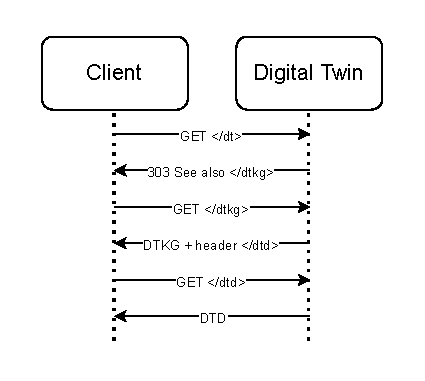
\includegraphics[width=\textwidth]{figures/hwodt/dtddtkg.pdf}
        \caption{}
        \label{fig:sequence-dtddtkg}
    \end{subfigure}
    \hfill
    \begin{subfigure}[t]{0.46\columnwidth}
        \centering
        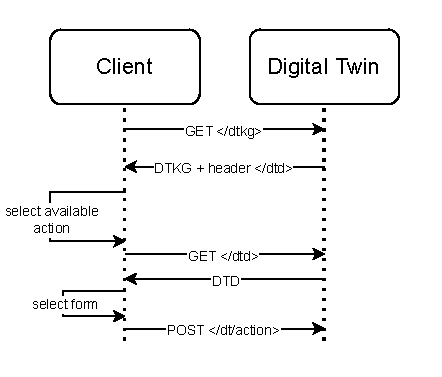
\includegraphics[width=\textwidth]{figures/hwodt/dtdactioncrop.pdf}
        \caption{}
        \label{fig:sequence-action}
    \end{subfigure}
    \caption{Interaction patterns to (a) access the \ac{DTD} and \ac{DTKG} and (b) invoke available actions on a \ac{DT} through the uniform interface and standard Web patterns.}
    \label{fig:sequence-interactions}
\end{figure}



Technically, since a \ac{DT} qualifies as a \emph{non-information resource}\footnote{For a discussion on information vs. non-information resources see \url{https://www.w3.org/TR/cooluris/} and \url{https://lists.w3.org/Archives/Public/www-tag/2005Jun/0039.html}}
the standard Web practice is returning a 303 (See Other) status code with the \textit{Location} HTTP header set to the \ac{URL} of the \ac{DTKG} information resource.
%
The \ac{URL} of the \ac{DTD} is linked in an HTTP Link Header with a custom relation type \texttt{dtd} in the response of the \ac{DTKG} GET request.
%
In this way, consumers can follow links between resources and access both \ac{DT} representations with standard Web interactions as shown in \Cref{fig:sequence-dtddtkg}.

Since the \ac{DTKG} evolves over time to reflect the \ac{PA} state, \acp{DT} are required to support a subscription \ac{API} to observe such changes (e.g., via WebSockets, long-polling, or WebSub~\cite{websub}).
Modeling the \ac{DTKG} as a Web resource also enables basic historicization using protocols like Memento~\cite{rfc7089}, if the \ac{DT} acts as a Memento TimeGate.

Finally, the \ac{API} may expose \ac{DT} actions that can be invoked by external consumers.
The \ac{DTKG} shows which actions are currently valid, while the \ac{DTD} describes how to request their execution to the \ac{DT}.
Consumers rely on both to interact and invalid actions should fail (e.g., with HTTP 403), ensuring consistency with the \ac{DT} model.
%
Figure \ref{fig:sequence-action} illustrates the interaction pattern to invoke an action on a \ac{DT}, by first checking its availability in the \ac{DTKG} and then following the affordance described in the \ac{DTD} to execute it.

%---------------------------------------------
\subsection{Ecosystem Services in the HWoDT}
\label{ssec:ecosystem-services}
%---------------------------------------------

In the proposal for realizing the \ac{HWoDT} ecosystem functionalities described in \Cref{chap:dte:dte} are implemented through a middleware:
%
the \emph{\ac{WoDT} Platform} aggregates data from registered \acp{DT} and exposes an \ac{API} that consumers can use to manage and interact with the ecosystem as a whole.

%........................................
\subsubsection{Managing the \acl{HWoDT}}
%........................................

The \ac{HWoDT} proposal assumes that \acp{DT} are existing, independently running software entities which implement the uniform interface presented in \Cref{ssec:uniform-interface}.
%
Hence, the \ac{DT} creation is handled by developers with their technology of choice, and adding it to an ecosystem is simply a matter of registering it to a \ac{WoDT} Platform. 
%
The platform exposes an \ac{API} that either managers, an external service or a \ac{DT} itself, can use to submit a \ac{DTD} to register a new \ac{DT} to the ecosystem.
The \ac{DTD} is then stored in a registry, which further allows it to be updated or removed if the \ac{DT} leaves the ecosystem.
%
Consumers can also use the registry \ac{API} to discover which \acp{DT} are in the ecosystem and to filter them based on metadata in the \ac{DTD}---e.g., they can discover if multiple \acp{DT} in the ecosystem model the same \ac{PA} filtering on the \ac{PA} identifier.

These simple operations are sufficient to manage the ecosystem. 
%
The \ac{DTD} is used in the registration process as it provides the necessary metadata to assess membership and compliance requirements as well as the \ac{API} description that the platform can use to interact with the \ac{DT} upon registration.
% 
Once registered, the platform uses the \ac{API} description within the \ac{DTD} to access and observe the \ac{DTKG}.  
It can also notify successful registration, enabling the \ac{DT} to record the platform \ac{URI} in its list of ecosystems updating its \ac{DTD} accordingly.

%..........................................
\subsubsection{Exploiting the \acl{HWoDT}}
%..........................................

By observing each individual \ac{DTKG}, the platform can cache the latest update and aggregate them to create a global \ac{DTE} \ac{KG} that can be exploited to implement ecosystem-level services for consumers.
%
The \ac{DTD} and \ac{DTKG} of each \ac{DT} are stored within the \ac{KG}, allowing queries to easily retrieve all available information about a \ac{DT}.
%
Each update of a \ac{DTKG} is processed and merged in the global \ac{KG} so that current representation of the whole ecosystem is always available to consumers.



The \ac{DTE} is a non-information resource and has a \ac{URI} which, when dereferenced, returns the global \ac{DTE} \ac{KG}\footnote{As the ecosystem \ac{KG} can be very large, returning the whole thing can be impractical. Alternatives include returning a partial representation with links to the \acp{DT} caches}.
%
Consumers can also \emph{query} the \ac{DTE} \ac{KG} through the \ac{WoDT} platform SPARQL endpoint.
%
This enables the extraction of selected information from the current state of all \acp{DT} in the ecosystem with a standard query language.

Finally, consumers may want to observe the evolution of the ecosystem \ac{KG}. The platform must then support an \ac{API} to receive subscription requests and send updates to observers.
%
Given the large nature of the \ac{DTE} \ac{KG}, consumers might not be interested in receiving \emph{all} updates. Hence, techniques for \ac{RDF} stream processing~\cite{barbieri2009www} might be more effective to support selective observation.

%======================================================
\section{A Prototype Framework for the HWoDT}
\label{sec:hwodt-impl}
%======================================================

To support the prototyping of heterogeneous \acp{DTE} based on the \ac{HWoDT} proposal, a set of tools is implemented aiming at the integration of existing \ac{DT} technologies.
%
The HWoDT framework is open source and available on GitHub\footnote{\url{https://github.com/Web-of-Digital-Twins}}. 

The software distribution includes a prototype \emph{\ac{WoDT} Platform} implementation and \emph{adapters} to implement the \ac{HWoDT} uniform interface for \acp{DT} developed with \azureTwin{}, \ditto{}, and the \ac{WLDT} framework (\Cref{sec:dte:engineering-dt:wldt-framework}).
%
The technology choice is meant to be representative of the state of the art as they differ in terms of functionalities, namely \azureTwin{} is a cloud platform, Ditto is an open-source platform, and \ac{WLDT} allows developing and deploying \acp{DT} as standalone software processes.
This section presents the overall architecture (\Cref{fig:abstract_arch}) and its implementation.


\begin{figure}
  \centering
  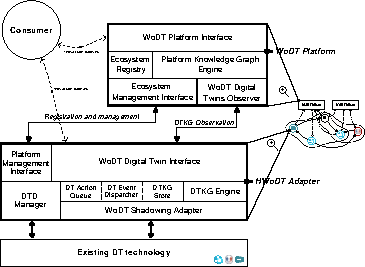
\includegraphics[width=0.8\columnwidth]{figures/hwodt/abstract_arch.pdf}
  \caption{Overall abstract architecture of the \ac{HWoDT} framework, showing the main functional modules. On the bottom existing \acp{DT} which, through the adapter, can implement the \ac{HWoDT} uniform interface and be integrated with a \ac{WoDT} platform.}
  \label{fig:abstract_arch}
\end{figure}



%----------------------------------------------
\subsection{A \ac{WoT}-compatible \acl{DTD}}
%----------------------------------------------

The \ac{DTD} is a central component in the design of the uniform interface of the \ac{HWoDT}.
%
Its design is inspired to the \ac{WoT} \ac{TD}, as an \ac{API} description of the functionalities offered by a \ac{DT}.

Although the \ac{WoT} explicitly reference \acp{DT} in its architectural patterns, the \ac{TD} alone does not support all the metadata that are needed in the proposed \ac{DTD}.
Hence, using \ac{WoT}-compliant mechanisms, \acp{TD} are extended to include the relevant metadata in order to qualify as a functional \ac{DTD} for a prototype implementation of the \ac{HWoDT}.
%
Namely, the \ac{TD} is extended using a custom \emph{\ac{WoDT} vocabulary}\footnote{\url{https://github.com/Web-of-Digital-Twins/wodt-vocabulary}}
which defines concepts to implement the \ac{DTD} and the \ac{DTKG}, as well as HTTP Link Headers relation types used in the interactions of the \ac{HWoDT} (see \Cref{ssec:uniform-interface}).
%
\Cref{lst:dtd-thing-model} shows a generic \ac{TM}~\cite{wot-td} that can be used to implement a valid \ac{DTD}. The \ac{DTD} must include:
\begin{itemize}
    \item the \ac{PA} identifier, 
    \item a link to the \ac{DTKG},
    \item an \texttt{observeallproperties} affordance to subscribe to updates of the \ac{DTKG}.
\end{itemize}

\lstinputlisting[
    label={lst:dtd-thing-model},
    caption={The Thing Model that Thing Descriptions must
    implement to be recognized as a valid \acl{DTD}.},
]{listings/hwodt/dtd.jsonld}


% \begin{figure}
%   \centering
%   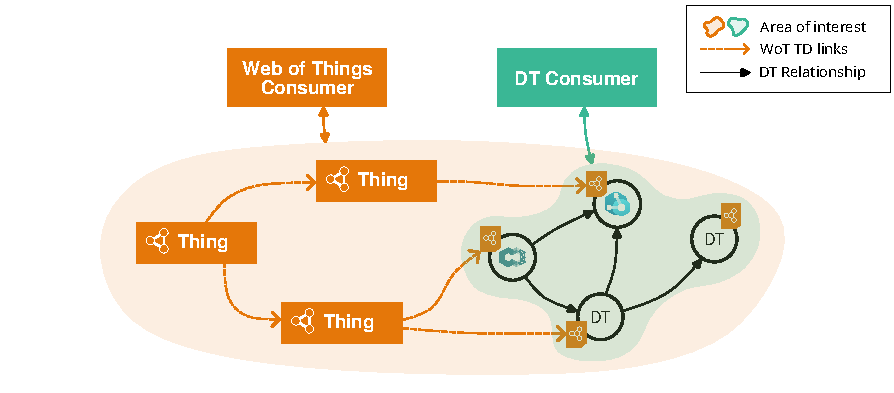
\includegraphics[width=\columnwidth]{figures/hwodt/wot-dt-mashups.pdf}
%   \caption{Keeping Digital Twin representations aligned with the \ac{WoT} Thing Description enables the creation of mixed mashups and interoperability with existing \ac{WoT} consumers.}
%   \label{fig:wot-dt-mashups}
% \end{figure}

The alignment with the \ac{WoT} is strategic for the \ac{DT} community as reusing the existing standard ensures compatibility and favors the development of application mashups.
%
The \ac{DTD} can be served by the \ac{DI} of a \ac{DT} to be discovered and consumed by existing \ac{WoT} clients (see \Cref{sec:dte:engineering-dt:physical-digital-adapters}).
%
Clients that have the capability to interpret the \ac{WoDT} vocabulary can then exploit the additional metadata to interact with the \ac{DT} as part of a \ac{HWoDT} ecosystem as shown in \Cref{fig:wot-dt-mashups}.

%-----------------------------
\subsection{HWoDT Adapters}
\label{ssec:adapters}
%------------------------------

\acp{DT} in a \ac{HWoDT} ecosystem must all adhere to the uniform interface, regardless of the technology used to implement them.
%
Adapting existing \ac{DT} technologies to the \ac{HWoDT} interface requires aligning data and interaction patterns.
%
To show that this alignment is achievable with configurable reusable components a set of \emph{adapters} is developed to integrate some mainstream technologies within a \ac{HWoDT} ecosystem.
%
All adapters support HTTP interactions and WebSocket-based \ac{DTKG} observation.
%
The abstract architecture followed by all adapters is shown in \Cref{fig:abstract_arch}, bottom.

%..............................................
\subsubsection{\azureTwin{} Adapter}
%..............................................

\azureTwin{} is Microsoft's domain-independent \ac{PaaS} \ac{DT} solution, supporting the management of multiple \acp{DT} connected within a \emph{twin graph}.

Creating \acp{DT} in \azureTwin{} requires defining their model using the \emph{\acf{DTDL}}, a custom JSON-LD format to specify properties, relationships, commands (actions) and telemetry (events) that describe a \emph{type} of \ac{DT}.
%
\ac{DTDL} models can then be used to create \ac{DT} instances.
%
Although the model closely aligns with the \ac{WoDT} model, the support of events and actions is partial\footnote{As of June 2025, commands can be defined but not invoked automatically, while telemetries are not used within \azureTwin{} \url{https://learn.microsoft.com/en-us/azure/digital-twins/concepts-models}} and relationships are limited to linking \acp{DT} within the same \azureTwin{} instance, which hence defines a closed homogeneous ecosystem.

The \azureTwin{} adapter is implemented as a middleware, connecting to an \azureTwin{} instance and mapping \acp{DT} to the \ac{HWoDT} uniform interface.
%
The adapter can be configured to select which \acp{DT} needs to be mirrored and specify the mapping from \ac{DTD} properties and relationships to produce the \ac{DTKG}. 
%
\Cref{fig:azure-adapter-c&c} shows the adapter architecture and the necessary components to connect to an \azureTwin{} instance.
%
The following Azure service pipeline must be set up to link the \azureTwin{} instance to the adapter:
\begin{itemize}
    \item \textit{Azure Event Grid} to capture and forward \azureTwin{} events;
    \item \textit{Azure Function} (\acl{FaaS}) to fetch the current \ac{DT} state and send it to the adapter via SignalR on every new event;
    \item \textit{Azure SignalR} to deliver \acp{DT} state updates to the adapter.
\end{itemize}

The adapter can be deployed either within the Azure cloud or is designed to automatically retrieve the \ac{DTDL} models, stored on \azureTwin{}, and convert them in valid \acp{DTD} for each \ac{DT} instance.
The adapter waits for SignalR events to receive \ac{DT} state updates generated by the Azure Function and convert them into \acp{DTKG} updates.

\begin{figure}
    \centering
    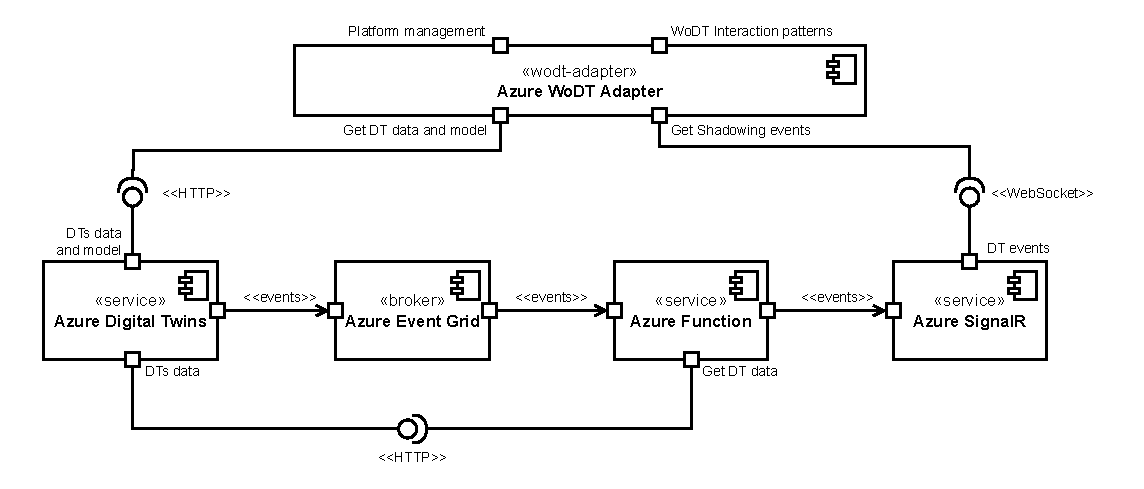
\includegraphics[width=\textwidth]{figures/hwodt/adtadapter-c&c.pdf}
    \caption{The \azureTwin{} adapter, implemented as a standalone component that maps specific instances of \acp{DT} hosted on an \azureTwin{} instance.}
    \label{fig:azure-adapter-c&c}
\end{figure}

%..............................................
\subsubsection{Eclipse Ditto Adapter}
%..............................................

\emph{Eclipse Ditto}, is an open-source \ac{DT} platform from the Eclipse Foundation. 
It abstracts each \ac{PA} as a \emph{Ditto Thing} and offers a Web-based layer for interacting with \ac{IoT} devices through their \acp{DT}.
%
A Ditto instance can manage multiple \acp{DT}, using a metamodel with:
\begin{itemize}
    \item \emph{Attributes} for static metadata,
    \item \emph{Features} which can group data (properties) and functionalities (messages).
\end{itemize}
Although lacking native support for relationships, actions, and events, these can be modeled using attributes (for links), consumer-to-\ac{DT} messages (for actions), and \ac{DT}-to-consumer messages (for events). Models can be defined via a custom JSON format or a (set of) \ac{WoT} \ac{TM}.

Eclipse Ditto is implemented with a microservice architecture. 
Despite Ditto being open-source and allowing the development of custom extensions, the prototype adapter is implemented as a custom external middleware that can be deployed to map one Ditto Thing to the \ac{HWoDT} uniform interface.
%
The middleware leverages Eclipse Ditto's native WebSocket interface to retrieve data and performs two key transformations: converting the \ac{WoT} \ac{TD} exposed by Ditto into a \ac{DTD}, and serializing \ac{DT} data into a \ac{DTKG}.
This process relies on a configurable mapping between Ditto features and their corresponding \ac{RDF} representations.

\begin{figure}[ht]
  \centering
  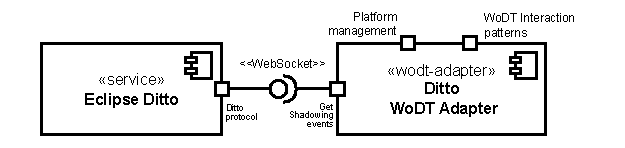
\includegraphics[width=0.8\columnwidth]{figures/hwodt/ditto-adapter-c&c.pdf}
  \caption{The Eclipse Ditto adapter, implemented as a standalone component that maps a specific instance of a \ac{DT} hosted on the Ditto platform.}
  \label{fig:ditto-adapter-c&c}
\end{figure}

%..............................................
\subsubsection{\acl{WLDT} Adapter}
%..............................................

The \emph{\acf{WLDT} framework} (\Cref{sec:dte:engineering-dt:wldt-framework}) enables the development of \acp{DT} as standalone software components deployable across cloud or edge environments.
%
Specifically, the adapter is implemented as a \ac{DiA}, used in the \ac{WLDT} architecture to represent digital interfaces through which the \ac{DT} can expose data for consumers.
%
The framework internal metamodel is already aligned with the \ac{HWoDT}, so no additional effort is required to map concepts.
The adapter is provided as a reusable Java library, which \ac{WLDT} developers can easily import into their projects and then configure the mapping towards the \ac{HWoDT} uniform interface leveraging the implementation of the necessary \ac{API} to manage the \ac{DTD} and \ac{DTKG}.

\begin{figure}[ht]
  \centering
  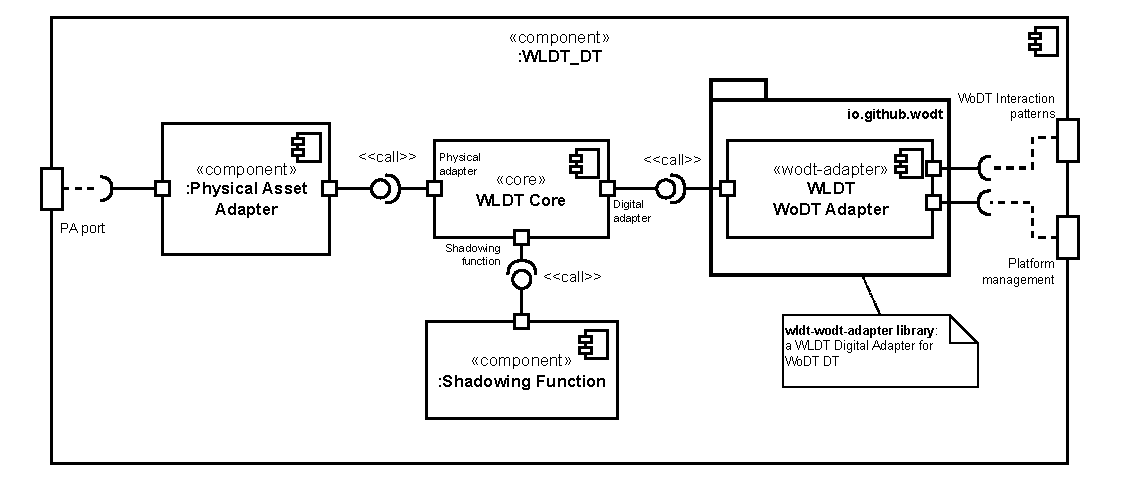
\includegraphics[width=\textwidth]{figures/hwodt/wldt-adapter-c&c.pdf}
  \caption{The architectural diagram of the \ac{WLDT} adapter, illustrating its integration with the other components of the framework.}
  \label{fig:wldt-adapter-c&c}
\end{figure}


%..............................................
\subsubsection{Implementing Custom Adapters}
%..............................................
The description of the adapters implemented in the prototype \ac{HWoDT} framework should be useful for any \ac{DT} developer wishing to implement a custom adapter for their own \ac{DT} or \ac{DT} technology. 
%
The idea of the \ac{HWoDT} is grounded on the fact that implementing such custom adapters is relatively straightforward and that the little effort spent in developing (or even less in configuring) them can bring benefits in the integration with the \ac{HWoDT} ecosystem.

To summarize, the steps to develop a custom adapter are: 
\begin{enumerate}
    \item understand how to map the concept of the original \ac{DT} model into the \ac{WoDT} metamodel;
    \item understand how to represent the state of the \ac{DT} with an evolving semantic representation for the \ac{DTKG};
    \item implement a module that can reactively produce the \ac{DTKG} whenever the \ac{DT} state is updated;
    \item implement a module that can serve the \ac{DTD} over HTTP, alongside the mandatory \ac{API} for \ac{DTKG} observation.
\end{enumerate}

%-----------------------------------
\subsection{The WoDT Platform}
%-----------------------------------

A prototype of a \ac{WoDT} Platform is implemented in Kotlin.
The platform implements the modules of the abstract architecture shown in \Cref{fig:abstract_arch}, top as shown in \Cref{fig:platform-c&c}.
%
Namely, the platform offers multiple interfaces for consumers: an HTTP \ac{API} for \ac{DTE} management (Ecosystem Management Interface) and one for \ac{KG} access with a SPARQL endpoint for read-only queries, as well as a WebSocket endpoint to observe ecosystem updates (\ac{WoDT} Platform Interface).

The platform can process the \ac{WoT}-based \ac{DTD} described above to register \acp{DT}.
When a registration requested is submitted, the platform:
\begin{enumerate}[label=\textbf{Step \arabic*}, leftmargin=5.3em]
    \item locates the \ac{DTKG} observation form (\texttt{observeallproperties}) and starts observing the \ac{DT} for updates;\label{step:observe-dtkg}
    \item notifies the \ac{DT} of successful registration to let it update its \ac{DTD} with the platform URI;\label{step:notification}
    \item maps the \ac{DT} \ac{URI} to a local cache URL;
    \item observes \ac{DTKG} updates and merges them into the \ac{DTE} \ac{KG} stored in memory with Apache Jena.
\end{enumerate}

%
The current prototype supports the observation of \ac{DTKG} through WebSockets for \ref{step:observe-dtkg} and implements \ref{step:notification} sending a request to a hardcoded \texttt{/platform} HTTP endpoint on the \ac{DT}.

Consumers can interact with the \acp{DTE} through the \ac{WoDT} platform
either through (possibly repeated) SPARQL queries to retrieve the information they need or by observing the whole \ac{KG} through WebSockets.
%
In the prototype, all observers receive the whole \ac{KG} whenever there is an update so that consumers don't need to have specific update handling logic.
%

\begin{figure}
  \centering
  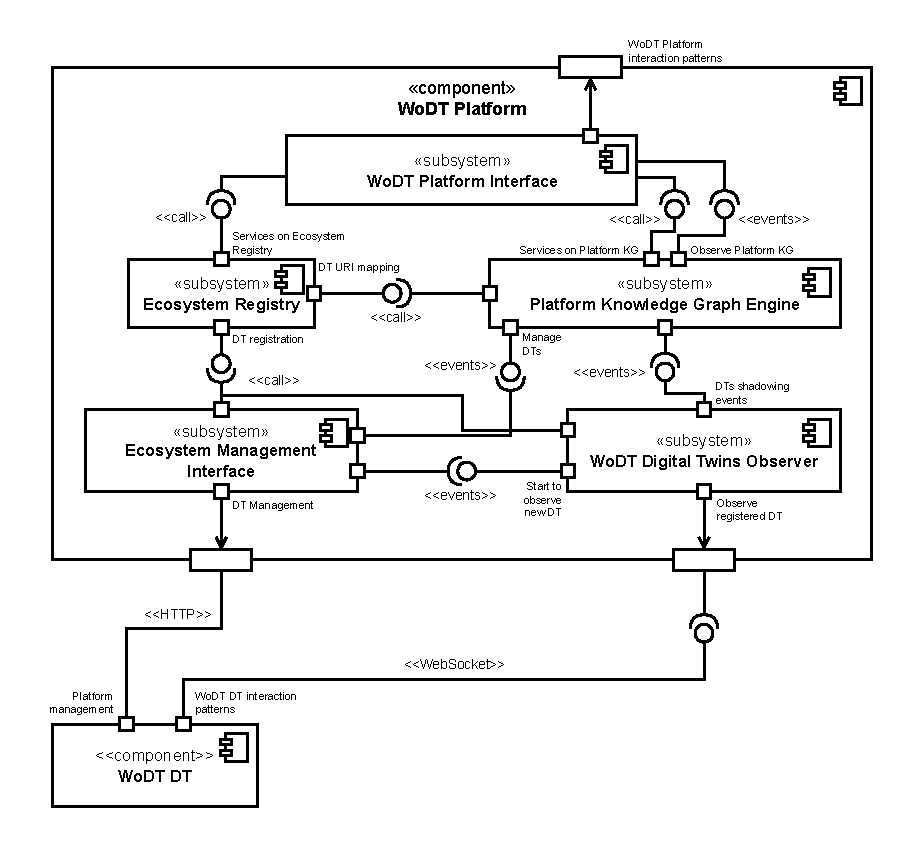
\includegraphics[width=\columnwidth]{figures/hwodt/platform-c&c.pdf}
  \caption{\ac{WoDT} Platform modules and interfaces, represented using components and connectors.}
  \label{fig:platform-c&c}
\end{figure}
